\documentclass[11pt,a4paper]{article}
\usepackage{url}
\usepackage{color}
\usepackage{graphicx}
\usepackage{cjhebrew}
\usepackage[T2A,OT2,OT1]{fontenc}
\usepackage{ucs}
\usepackage{CJKutf8}

\usepackage{subfigure}
\usepackage{floatrow}
\usepackage{multirow}
\usepackage[hebrew,english]{babel}

\usepackage{times}
\usepackage{latexsym}
\usepackage{draftwatermark}
\usepackage{acl2014}
\usepackage[footnotesize]{caption}

\newcommand{\heb}[1]{%
  \foreignlanguage{hebrew}{#1} }

\newcommand\cyr{%
\renewcommand\rmdefault{wncyr}% \renewcommand\sfdefault{wncyss}%
\renewcommand\encodingdefault{OT2}%
\normalfont
\selectfont}
\DeclareTextFontCommand{\textcyr}{\cyr}

\newcommand{\ddcomment}[1]{\textcolor{red}{[$^{\textsc{D}}_{\textsc{D}}$ #1]}}
\newcommand{\spcomment}[1]{\textcolor{blue}{[$^{\textsc{S}}_{\textsc{P}}$ #1]}}
\newcommand{\jmcomment}[1]{\textcolor{magenta}{[$^{\textsc{J}}_{\textsc{M}}$ #1]}}
\newcommand{\eat}[1]{\ignorespaces}
\newcommand{\cyrsmb}{\char126}

\newcommand{\query}[1]{\texttt{#1}}

\setlength\titlebox{6.5cm}    % Expanding the titlebox

\title{Enhanced Search with Wildcards and Morphological Inflections\\in the Google Books Ngram Viewer}

\author{Jason Mann, David Zhang, Lucille Yang, Dipanjan Das and Slav Petrov\\
	Google Inc. \\
	{\tt jcm2207@columbia.edu, dzhang21@gmail.com, ly77@cornell.edu}\\
	{\tt \{dipanjand,slav\}@google.com}}


\date{}

\begin{document}
\maketitle

\begin{abstract}

We present a new version of the Google Books Ngram Viewer, which plots
the frequency of words and phrases over the last five
centuries; its data encompasses 6\% of the world's published books.
The new Viewer adds three features for more powerful search: wildcards,
morphological inflections, and capitalization. These additions allow
the discovery of patterns that were previously difficult to find
and further facilitate the study of linguistic trends in printed text.

\end{abstract}

\section{Introduction}

The Google Books Ngram project facilitates the analysis of cultural, social and linguistic trends through five centuries of written text in eight languages. The Ngram Corpus \cite{culturomics,lin2012syntactic} consists of words and phrases (i.e., ngrams) and their usage frequency over time; it is freely available for download. The interactive Ngram Viewer\footnote{See \url{http://books.google.com/ngrams}.} allows users to retrieve and plot the frequency of multiple ngrams on a simple webpage. The Viewer is widely popular and can be used to efficiently explore and visualize patterns in the underlying ngram data. For example, the ngram data has been used to detect emotion trends in 20th century books \cite{acerbi.etal.2013}, to analyze text focusing on market capitalism throughout the past century \cite{Schulz2013}, detect social and cultural impact of historical personalities \cite{skiena.ward.2013}, or to analyze the correlation of economic crises with a literary `misery index' reflected in printed text during crises periods \cite{bentley.et.al.2014}.

\begin{figure}[t]
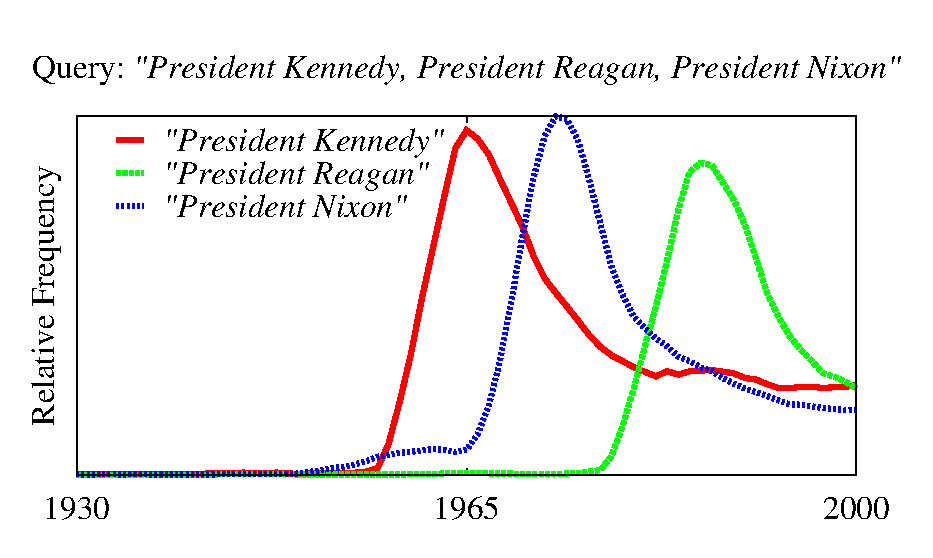
\includegraphics[width=\columnwidth]{graphs/kenreanixon}
\caption{\label{fig:manual}Mention frequencies for three different American presidents queried one-by-one.
\vspace{-1.5em}}
\end{figure}

A limitation of the Viewer, however, is that all the reasoning has to be done by the user, and only individual, user-specified ngrams can be retrieved and plotted. For example, to compare the popularity of different presidents, one needs to come up with a list of presidents and then search for them one-by-one. The result of the query `\query{President Kennedy, President Nixon, President Reagan}' is shown in Figure~\ref{fig:manual}. To determine the most popular president, one would need to search for all presidents, which is cumbersome and should ideally be automated.



In this paper, we therefore present an updated version of the Viewer that enhances its search functionality. We introduce three new features that automatically expand a given query and retrieve a collection of ngrams, to facilitate the discovery of patterns in the underlying data. First, users can replace one query term with a placeholder symbol `\query{*}' (wildcard, henceforth), which will return the ten most frequent expansions of the wildcard in the corpus for the specified year range. 
%Figure~\ref{fig:examples}(a) shows the automatically discovered increase in references to the University of California. 
Second, by adding a specific marker to any word in a query (`\query{\_INF}'), ngrams with all morphological inflections of that word will be retrieved. 
%Figure~\ref{fig:examples}(b) shows the four inflected forms of the word book in the ngram `book a hotel'.
Finally, the new Viewer supports capitalization searches, which return all capitalization variants of the query ngram. Figure~\ref{fig:examples} provides examples for these three new types of queries.
%Figure~\ref{fig:examples}(c) shows the decline in the camel-case spelling of the surname Fitzgerald.
% Slav: we could discuss the examples in Fig. 1 here.

While it is fairly obvious how the above search features can be implemented via brute-force computation, supporting an interactive application with low latency necessitates some precomputation. In particular, the wildcard search feature poses some challenges because the most frequent expansions depend on the selected year range (consider the frequency with which presidents are mentioned during different decades, for example). To this end, we provide details on our system architecture in \S\ref{sec:overview}  and discuss how the new search features are implemented in \S\ref{sec:features}.
% We could add a sentence summarizing how we deal with wildcards here.
In addition, we present an overhaul of the Ngram Viewer's user interface with interactive features that allow for easier management of the increase in data points returned.


\begin{figure}[!t]
\vspace{-0.5em}
\begin{subfigure}
  \centering
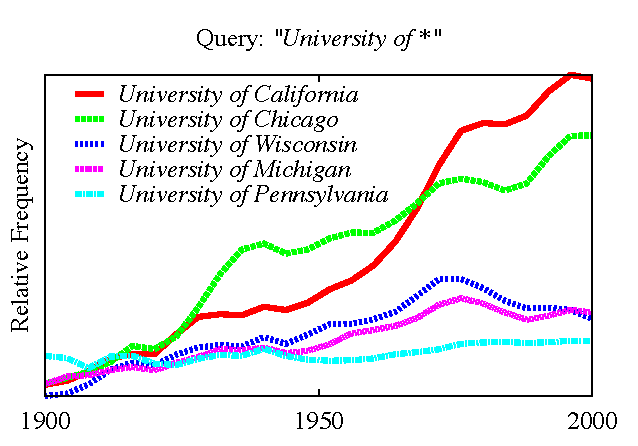
\includegraphics[width=\columnwidth]{graphs/university}\\
\end{subfigure}%
\vspace{-1em}
\begin{subfigure}
\centering
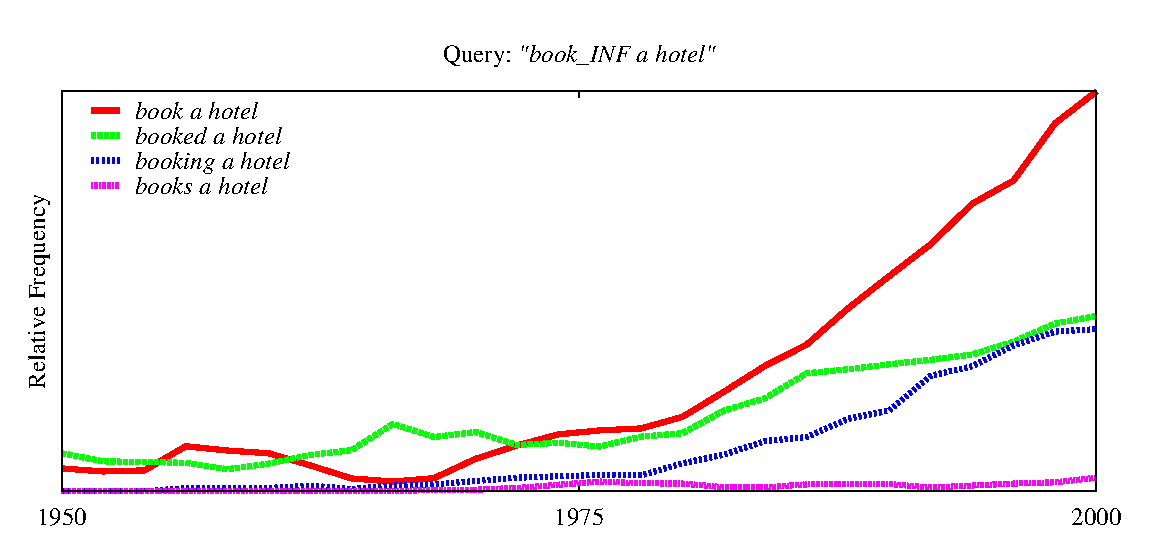
\includegraphics[width=\columnwidth]{graphs/book}\\
\end{subfigure}%
\vspace{-1em}
\begin{subfigure}
\centering
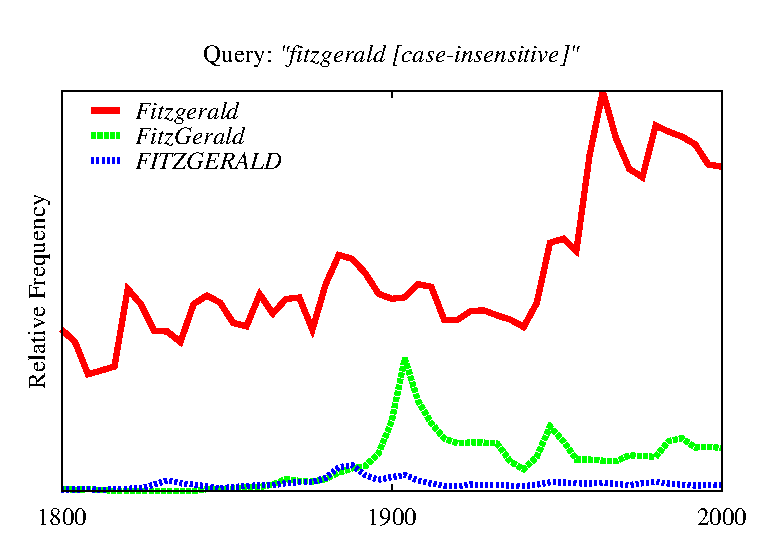
\includegraphics[width=\columnwidth]{graphs/fitzgerald}\\
\end{subfigure}
\caption{In the new enhanced search features of the Ngram Viewer presented here, a single query is automatically expanded to retrieve multiple related ngrams. From top to bottom, we show examples of the wildcard operator (`\query{*}'), the `\query{\_INF}' marker that results in morphological inflections, and the case insensitive search functionality. \label{fig:examples} We show fewer results in this figure than the ones returned by the Ngram Viewer due to space considerations.
\vspace{-1.5em}}
\vspace{-1em}
\end{figure}

Detailed analysis and interpretation of trends uncovered with the new search interface is beyond the scope of this paper. We highlight some interesting use cases in \S\ref{sec:usecases}; many of the presented queries were difficult (or impossible) to execute in the previous versions of the system.
 We emphasize that this demonstration updates only the Viewer, and provides tools for easier analysis of the underlying corpora. The ngram corpora themselves are not updated.
 \eat{For example, to normalize for morphological inflections or casing, the frequencies of multiple ngrams can be aggregated via a (right) mouse-click. Additionally, lines can be highlighted or faded (via hovering or mouse-clicks) to focus on particular ngrams and make trends more apparent.}




\section{System Overview}
\label{sec:overview}

We first briefly review the two editions of the Ngram Corpus \cite{culturomics,lin2012syntactic} and then describe the extensions to the architecture of the Viewer that are needed to support the new search features.


\subsection{The Ngram Corpus}
	The Google Books Ngram Corpus\footnote{Downloadable from \texttt{https://books.google.com/} \texttt{ngrams/datasets}.} provides ngram counts for eight different languages over more than 500 years; additionally, the English corpus is split further into British vs. American English and Fiction to aid domain-specific analysis. This corpus is a subset of all books digitized at Google and represents more than 6\% of all publicized texts \cite{lin2012syntactic}. Two editions of the corpus are available: the first edition dates from 2009 and is described in \newcite{culturomics}; the second edition is from 2012 and is described in \newcite{lin2012syntactic}. The new search features presented here are available for both editions.

\newcite{culturomics} extract ngrams for each page in isolation. More specifically, they use whitespace tokenization and extract all ngrams up to length five. These ngrams include ones that potentially span sentence boundaries, but do not include ngrams that span across page breaks (even when they are part of the same sentence).
\newcite{lin2012syntactic} on the other hand perform tokenization, text normalization and segmentation into sentences. They then add synthetic \textsf{\textsc{\_start\_}} and \textsf{\textsc{\_end\_}} tokens to the beginning and end of the sentences to enable the distinction of sentence medial ngrams from those near sentence boundaries. They also ensure that sentences that span across page boundaries are included. Due to these differences, as well as the availability of additional book data, improvements to the optical character recognition algorithms and metadata extraction for dating the books, the ngrams counts from the two editions are not the same.

The edition from \newcite{lin2012syntactic} additionally includes syntactic ngrams. The corpus is tagged using the universal part-of-speech (POS) tag set of \newcite{petrov2012universal}: \query{NOUN} (nouns), \query{VERB} (verbs), \query{ADJ} (adjectives), \query{ADV} (adverbs), \query{PRON} (pronouns), \query{DET} (determiners and articles), \query{ADP} (prepositions and postpositions), \query{CONJ} (conjunctions). Words can be disambiguated by their POS tag by simply appending the tag to the word with an underscore (e.g. \texttt{book\_NOUN}) and can also be replaced by POS tags in the ngrams, see \newcite{lin2012syntactic} for details. The corpus is  parsed with a dependency parser and head-modifier syntactic relations between words in the same sentence are extracted. Dependency relations are represented as `\query{=>}' in the corpus. Our new enhanced search features for automatic expansions can also be applied to these syntactic ngrams. In fact, some of the most interesting queries use expansions to automatically uncover related ngrams, while using syntax to focus on particular patterns.

The Viewer supports the composition of ngram frequencies via arithmetic operators. Addition (\query{+}), subtraction (\query{-}) and division (\query{/}) of ngrams are carried out on a per year basis, while multiplication (\query{*}) is performed by a scalar that is applied to all counts in the time series. Where ambiguous, the wildcard operator takes precedence over the multiplication operator. Parentheses can be used to disambiguate and to force the interpretation of a mathematical operation.

\begin{figure}[!t]
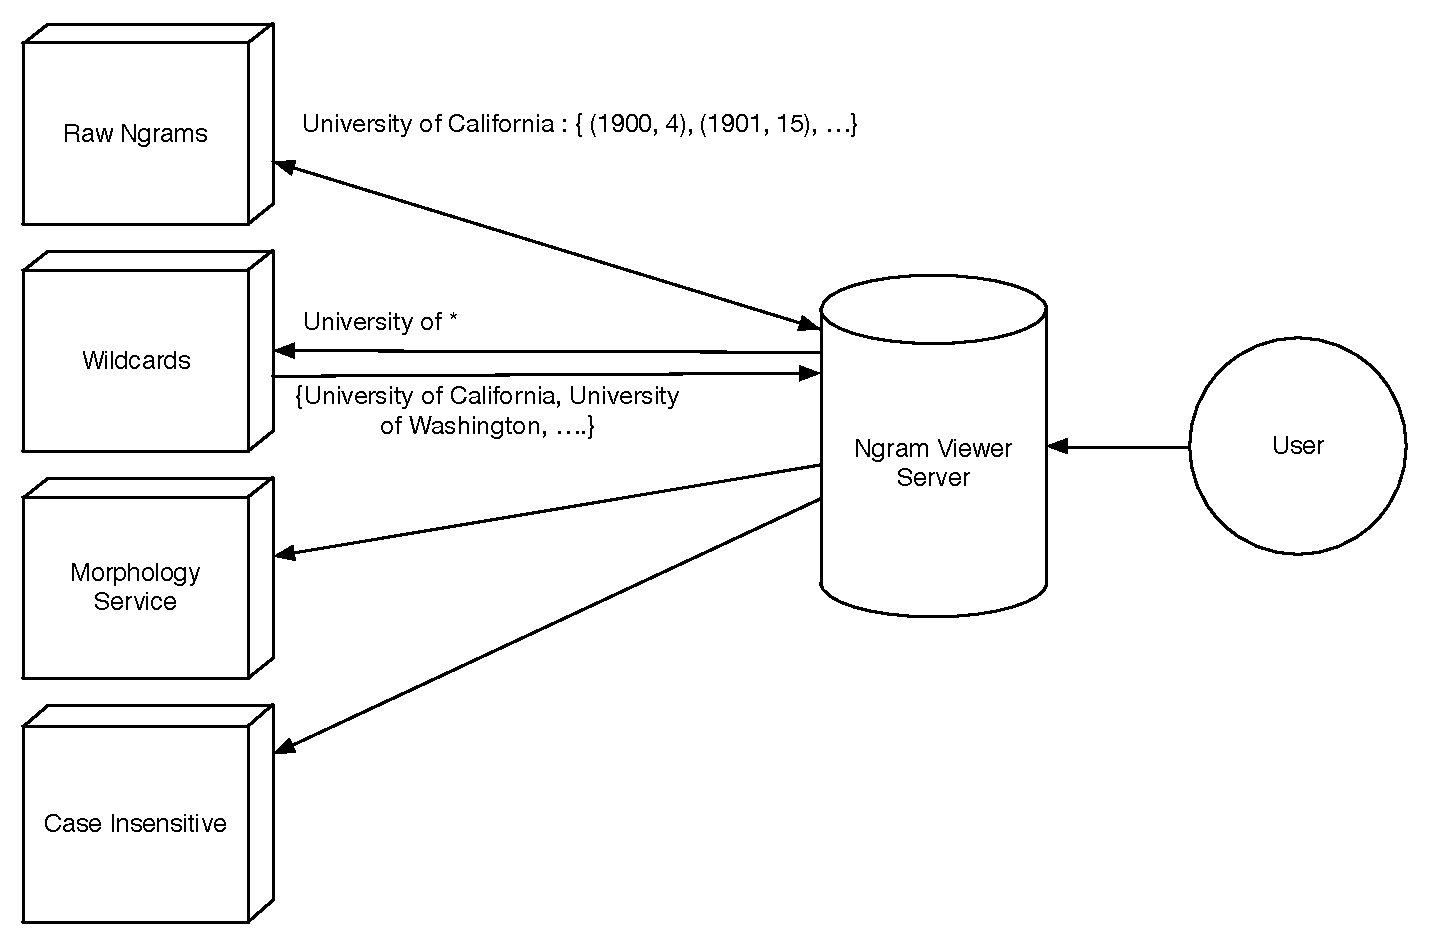
\includegraphics[width=\columnwidth,keepaspectratio=true]{system_architecture}
\vspace{-2.5em}
\caption{\label{fig:architecture}Overview of the Ngram Viewer architecture.\vspace{-1.5em}}
\end{figure}


\eat{\begin{figure*}[!t]
\centering
\addtolength{\subfigcapskip}{-0.2cm}
\hspace*{-0.5cm}
\subfigure[]{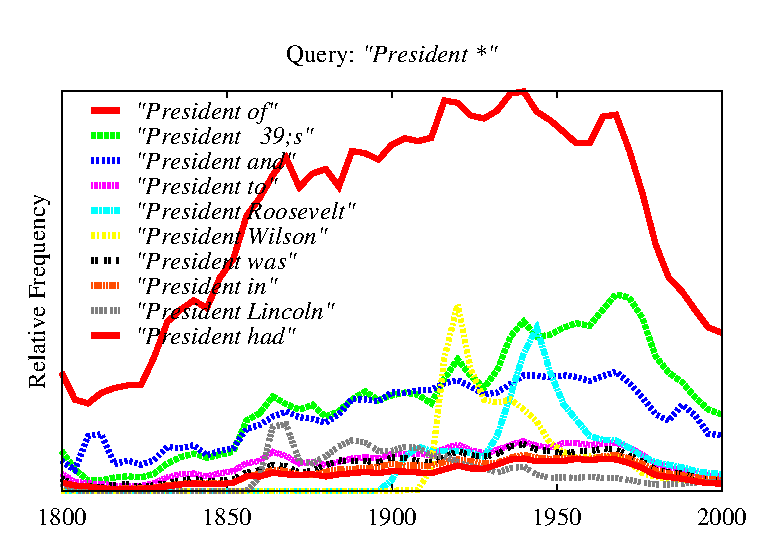
\includegraphics[width=0.49\textwidth]{graphs/president*_all}}
\hspace*{0.1cm}
\subfigure[]{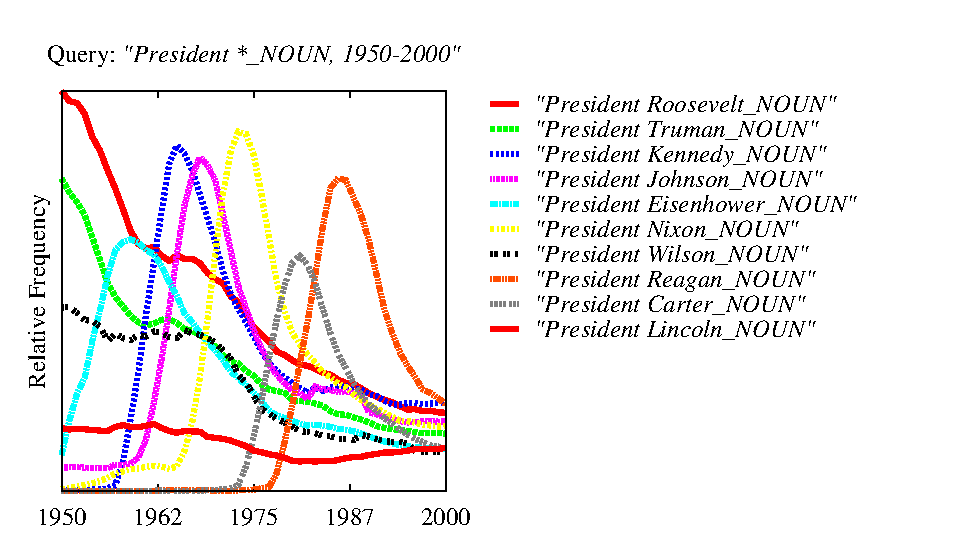
\includegraphics[width=0.49\textwidth]{graphs/President*1950}}

\hspace*{-0.5cm}\vspace*{-0.5cm}
\subfigure[]{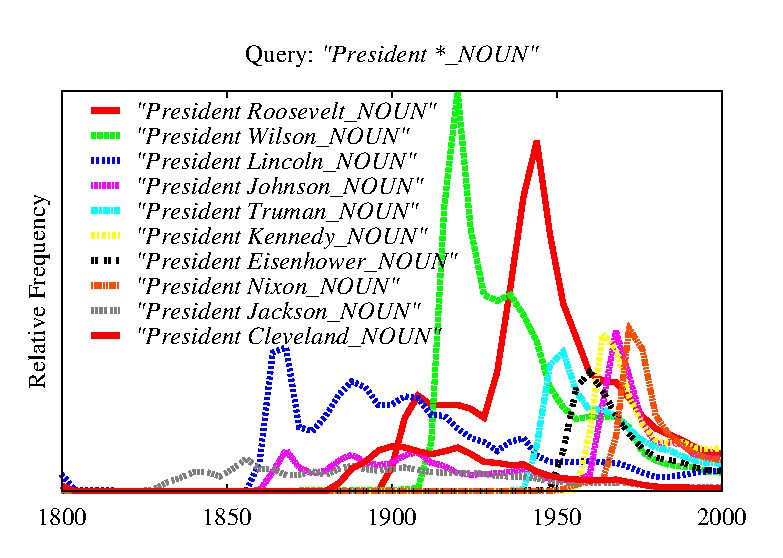
\includegraphics[width=0.69\textwidth]{graphs/President*1800}}
\hspace*{0.1cm}
\parbox[b][]{.28\textwidth}%
{\RawCaption{\caption{\label{fig:presidents}
Specification of a POS tag along with the wildcard operator results in more
specific results, as shown in (b) and (c).}}}
\end{figure*}}

\begin{figure*}[!t]
\vspace{-0.1in}
\centering
\addtolength{\subfigcapskip}{-0.2cm}
\hspace*{-0.5cm}
\subfigure{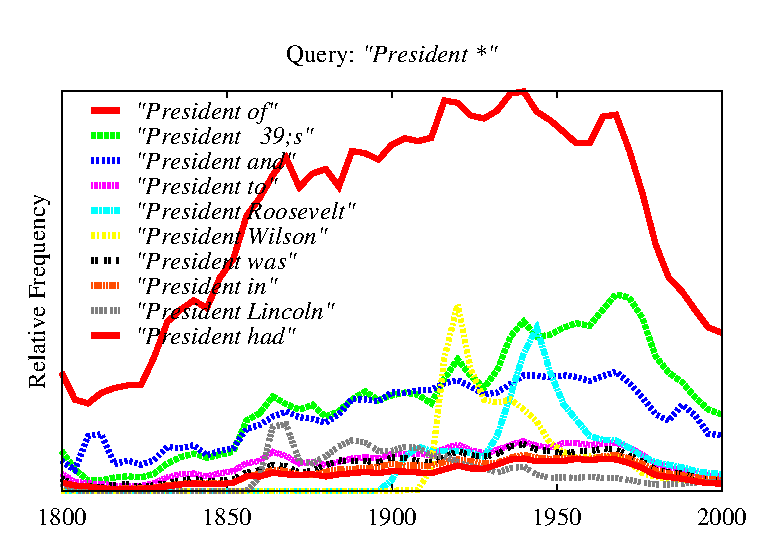
\includegraphics[width=0.33\textwidth]{graphs/president*_all}}
\subfigure{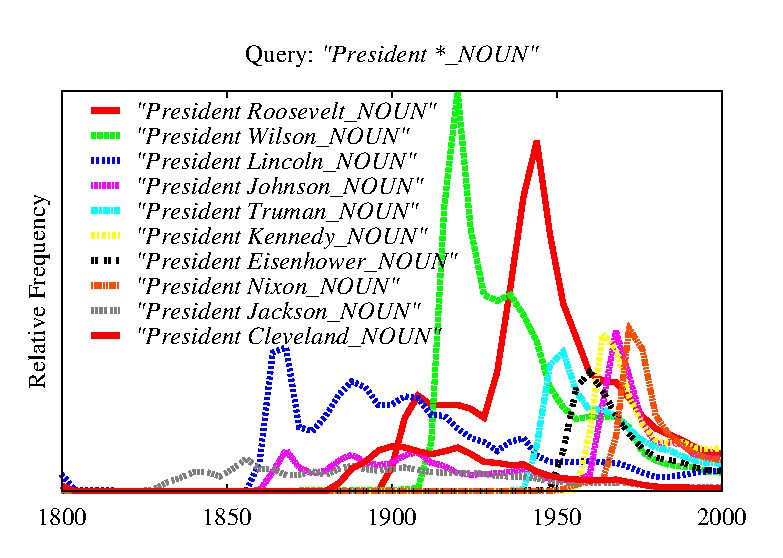
\includegraphics[width=0.33\textwidth]{graphs/President*1800}}
\subfigure{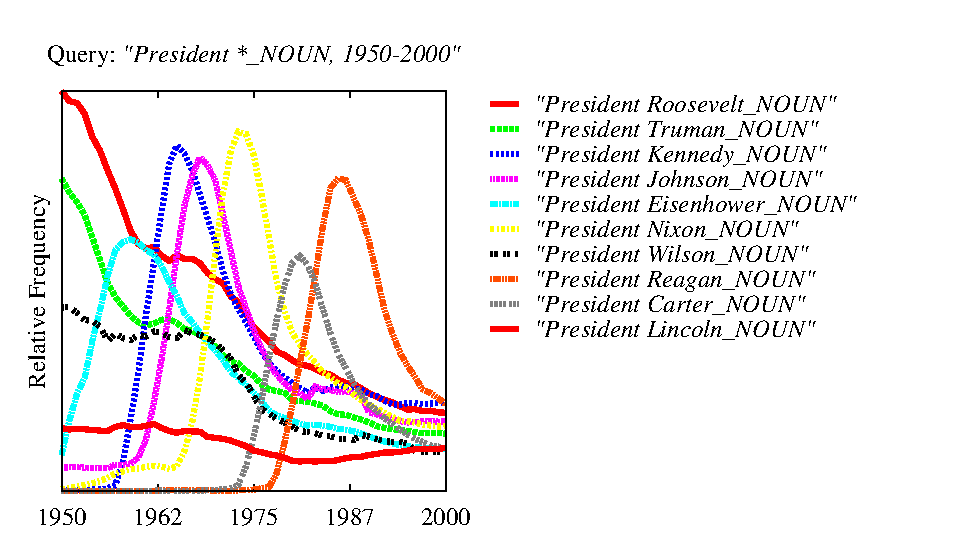
\includegraphics[width=0.33\textwidth]{graphs/President*1950}}
\caption{\label{fig:presidents}
Different wildcard queries for bigrams starting with \query{President}. Specification of a POS tag along with the wildcard operator results in more
specific results, and the results vary depending on the selected yaer range.}
\vspace{-0.1in}
\end{figure*}


\subsection{Architecture}
The Ngram Viewer provides a lightweight interface to the underlying ngram corpora. In its basic form, user requests are directed through the server to a simple lookup table containing the raw ngrams and their frequencies. This data flow is displayed in the top part of Figure~\ref{fig:architecture} and is maintained for queries that do not involve the new expansion features introduced in this work.

The expansion queries could in principle be implemented by scanning the raw ngrams on the fly and returning the matching subset: to answer the query `\query{President *}', one would need to obtain all bigrams starting with the word \query{President} (there are 23,693) and extract the most frequent ten. Given the large number of ngrams, such an approach turns out to be too slow for an interactive application. We therefore pre-compute intermediate results that can be used to more efficiently retrieve the results for expansion queries. The intermediate results are stored in additional lookup tables (shown at the bottom in Figure~\ref{fig:architecture}). When the user executes an expansion search, the query is first routed to the appropriate lookup table which stores all possible expansions (including expansions that might not appear in the corpus).  These expanded ngrams are then retrieved from the raw ngram table, sorted by frequency and returned to he user.
%For example, the intermediate results table for the morphological variants search contains inflected forms for all unigrams. These inflected forms are substituted for the selected query term and the resulting ngram is looked up in the raw ngram table.
We describe the intermediate results tables and how they are generated in the next section.

Note that we only support one expansion operation per query ngram. This is needed in order to avoid the combinatorial explosion that would result from mixing multiple expansion operators in the same query.


\section{New Features}
\label{sec:features}
The three new search features are implemented via the same two-step approach. As shown in Figure~\ref{fig:architecture}, we add three new lookup tables that store intermediate results needed for efficiently supporting the new search types. In all cases the lookup tables provide a set of possible expansions that are then retrieved in the original raw ngram table. Below we describe how these intermediate results are generated and how they are used to retrieve the final results.

\subsection{Wildcards}
\label{sec:wildcards}
	Wildcards provide a convenient way to automatically retrieve and explore related ngrams. Because of the large number of possibilities that can fill a wildcard slot, returning anything but the top few expansions is likely to be overwhelming. We therefore return only the ten most frequent expansions. Determining the most frequent expansions is unfortunately computationally very expensive because of the large number of ngrams; the query `\query{the *}' for example has 2,353,960 expansions.

 To avoid expensive on-the-fly computations, we precompute the most frequent expansions for all possible queries. The problem that arises is that the ten most frequent expansions depend on the selected year range. Consider the query `\query{President *}'; we would like to be able get the correct result for any year range. Since our data spans more than 500 years, precomputing the results for all year ranges is not a possibility. Instead, we compute the possible wildcard expansions for each year. The top expansions for the entire range are then taken from the union of top expansions for each year. This set is at most of size $10n$ (where $n$ is the year range) and in practice typically a lot smaller. Theoretically it is possible for this approximation to miss an expansion that is never among the top ten for a particular year, but is cumulatively in the top ten for the entire range. This would happen if there were many spikes in the data, which is not the case.
% Slav: the following sentence could be deleted.
%To be safe, we define the wildcard search to return the top ten expansions where each of them is at least in one year among the ten most frequent expansions.

	To make the wildcard expansions more relevant, we filter expansions that consist entirely of punctuation symbols. To further narrow down the expansions and focus on particular patterns, we allow wildcards to be qualified via POS tags. Figure~\ref{fig:presidents} shows some example wildcard queries involving bigrams that start with the word `\query{President}.' See also Table \ref{tab:wildcard} for some additional examples. Note that it is possible to replace POS tags with wildcards (e.g., \query{cook\_*}) which will find all POS tags that the query word can take.

\begin{table*}[!t]
\small
\centering
\begin{tabular}{|c|c|}
\hline
\textbf{Query}	& \textbf{Possible Replacements}	\\ \hline \hline
\query{* 's Theorem}				& \begin{tabular}[c]{@{}c@{}}\query{Lagrange 's Theorem, Gauss 's Theorem,} \\ \query{Euler 's Theorem, Pascal 's Theorem}	\end{tabular}\\ \hline
\query{War=>*\_NOUN}	& 
\begin{tabular}[c]{@{}c@{}} \query{ War=>World\_NOUN, War=>Civil\_NOUN, }\\\query{War=>Second\_NOUN, War=>Cold\_NOUN}  \end{tabular} \\ \hline
\query{\textcyr{lubov\cyrsmb}\_INF	}	& \query{\textcyr{lubil, lublu, lubit, lubit\cyrsmb, lubila, lubimy{\u i}, lubish\cyrsmb}} \\ \hline
\query{book\_INF		}	& \query{book, books, booked, booking    } \\ \hline
\query{book\_INF\_NOUN		}	& \query{book, books     } \\ \hline
\query{cook\_*		}	& \query{cook\_NOUN, cook\_VERB     } \\ \hline
\begin{tabular}[c]{@{}c@{}} \query{the cook} (case insensitive)\end{tabular} & \query{THE COOK, the cook, The Cook, the Cook, The cook  } 	  \\ \hline
\end{tabular}
\caption{\label{tab:wildcard}
Examples expansions for wildcard, inflection, and capitalization queries.}
\end{table*}

\subsection{Morphological Inflections}\label{sec:morph}
When comparing ngram frequencies (especially across languages, but also for the same language), it can be useful to examine and potentially aggregate the frequencies of all inflected forms. This can be accomplished by manually deriving all inflected forms and then using arithmetic operations to aggregate their counts. Our new inflected form search accomplishes this automatically. By appending the keyword \query{\_INF} to a word, a set of ngrams with all inflected forms of the word will be retrieved. To generate the inflected forms we make use of Wiktionary\footnote{See \url{http://www.wiktionary.org/}. Because Wiktionary is an evolving resource, results for a particular query may change over time.} and supplement it with automatically generated inflection tables based on the approach of \newcite{durrett2013supervised}.

Because there are at most a few dozen inflected forms for any given word, we can afford to substitute and retrieve all inflections of the marked word, even the ones that are not grammatical in a given ngram context. This has the advantage that we only need to store inflected forms for individual words rather than entire ngrams. If a generated ngram has no support in the corpus, we simply omit it from the final set of results. We do not perform any additional filtering; as a result, an inflection search can produce many results, especially for morphologically rich languages like Russian. We have therefore updated the user interface to better deal with many data lines (\S\ref{sec:usecases}).

\subsection{Capitalization}

By aggregating different capitalizations of the same word, one can normalize between sentence-initial and sentence-medial occurrences of a given word. A simple way to accomplish this is by searching for a lowercased, capitalized and all caps spelling of the query. This however can miss CamelCase spelling and other capitalization variants (consider \query{FitzGerald} for example). It is of course not feasible to try all case variants of every letter in the query. Instead, we perform an offline precomputation step in which we collect all ngrams that map to the same lowercased string. Due to scanning errors and spelling mistakes there can be many extremely rare capitalization variants for a given query. We therefore filter out all variants that have a cumulative count of less than 1\% of the most frequent variant for a given year range. Capitalization searches are enabled by selecting a case-insensitive check box on the new interface.

\eat{\section{User Interface}
\label{sec:interface}}

\eat{\begin{figure}[!t]
\centering
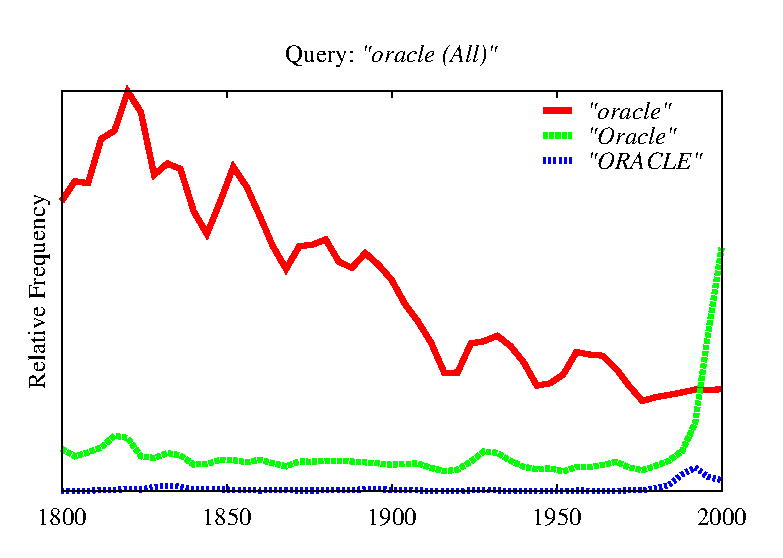
\includegraphics[width=\columnwidth]{graphs/oracle}
\caption{\label{fig:oracle} Discovery of Capitalization usage.
\vspace*{-1.5em}}
\end{figure}}


\section{Use Cases}
\label{sec:usecases}

The three features introduced in this paper represent a major extension of the capabilities of the Ngram Viewer. While the second edition of the Ngram Corpus \cite{lin2012syntactic} introduced syntactic ngrams, the functionality of the Viewer had remained largely unchanged since its first launch five years ago. Together, the updated Corpus and Viewer enable a much more detailed analysis of the underlying data. Below we provide some uses cases highlighting the ways in which sophisticated queries can be crafted. While the results produce some intriguing patterns, we leave their analysis to the experts.

\begin{figure*}[t]
\vspace{-0.1in}
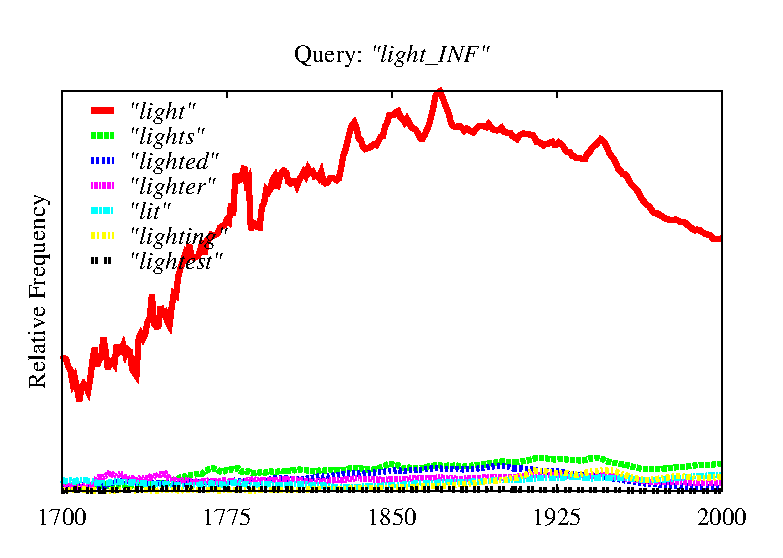
\includegraphics[width=.48\textwidth]{graphs/light_INF}
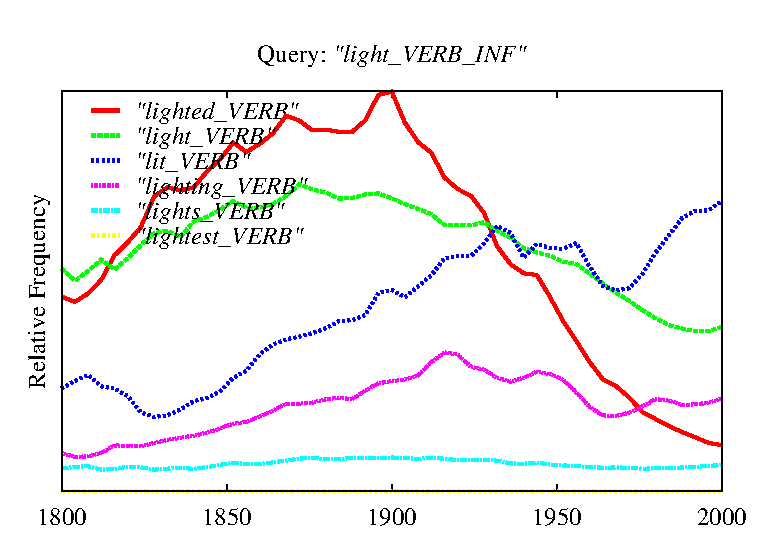
\includegraphics[width=.48\textwidth]{graphs/light_INF_VERB}
\vspace*{-1em}
\caption{\label{fig:light} Comparison of specification of POS tag in wildcard search.}
\end{figure*}

\begin{table*}[ht]
\small
\centering
\begin{tabular}{|c|c|c|c|c|c|c|c|c|c|}
\hline
\textbf{English} & \textbf{American} & \textbf{British} & \multirow{2}{*}{\textbf{German}} & \multirow{2}{*}{\textbf{French}} & \multirow{2}{*}{\textbf{Russian}} & \multirow{2}{*}{\textbf{Italian}} & \textbf{Chinese} & \multirow{2}{*}{\textbf{Spanish}} & \multirow{2}{*}{\textbf{Hebrew}} \\
\textbf{(All)} &  \textbf{English} & \textbf{English} & & & & &  \textbf{(Simplified)} & &  \\
\hline
\query{drinks} & \query{drinks} & \query{drinks} & \query{trinkt} & \query{boit} & \textcyr{p\cyrsmb \"et} & \query{beve} & \begin{CJK}{UTF8}{gbsn}  喝 \end{CJK} & \query{bebe} & \heb{התש}\\
\hline \hline
\query{water}&\query{water}&\query{water}&\query{Bier}  &\query{vin}  &\textcyr{on}       &\query{vino}    &\begin{CJK}{UTF8}{gbsn}酒  \end{CJK}&\query{agua}   &\heb{ןיי}\\
\query{wine} &\query{wine} &\query{wine} &\query{Kaffee}&\query{sang}  &\textcyr{cha{\u i}}&\query{acqua}   &\begin{CJK}{UTF8}{gbsn}茶  \end{CJK}&\query{vino} &\heb{םימ}\\
\query{milk}&\query{coffee}&\query{tea}  &\query{Wein}  &\query{eau} &\textcyr{vodu}     &\query{sangue}  &\begin{CJK}{UTF8}{gbsn}水  \end{CJK}&\query{sangre}   &\heb{ה}  \\
\query{coffee}&\query{beer}&\query{blood}&\query{Wasser}&\query{cafe}&\textcyr{On}       &\query{birra}   &\begin{CJK}{UTF8}{gbsn}咖啡\end{CJK}&\query{vaso}   &\heb{סוכ}\\
\query{beer} &\query{milk} &\query{beer} &\query{Tee}   &\query{verre}   &\textcyr{vino}  & \query{caff\'e} &\begin{CJK}{UTF8}{gbsn}人  \end{CJK}&\query{cerveza}&\heb{הת}\\\hline 
\end{tabular}
\caption{\label{tab:drink}Comparison of the top modifiers of the verb \query{drinks} in all corpora, retrieved via the query \query{drinks\_VERB=>*\_NOUN} and equivalents in the other languages. The modifiers can appear both in subject and in object position because we have access only to unlabeled dependencies.}
\end{table*}

Since we have made no modifications to the underlying raw ngrams, all of the plots in this paper could have also been generated with the previous version of the Viewer. They would however have required the user to manually generate and issue all query terms. For example, Figure~\ref{fig:manual} shows manually created queries searching for specific presidents; contrarily, Figure \ref{fig:presidents} shows single wildcard queries that automatically retrieve the ten most frequently mentioned presidents and uncover additional trends that would have required extra work on behalf of the user.

The wildcard feature used on its own can be a powerful tool for the analysis of top expansions for a certain context.  Although already useful on its own, it becomes really powerful when com with POS tags. The user can attach an underscore and POS tag to either a wildcard-based or inflection-based query to specify that the expansions returned should be of a specific part of speech. Compare the utility of the generic wildcard and a search with a noun part-of-speech specification in a query examining president names, `\query{President *}' vs. `\query{President *\_NOUN}' shown in Figure \ref{fig:presidents}. The former gives a mixture of prepositions, particles, and verbs along with names of presidents, and because the latter specifies the noun tag, the top expansions turn out to be names and more in line with the intention of the search. Also, note in Figure \ref{fig:presidents} the difference in expansions that searching over two different time ranges provides. In Table~\ref{tab:drink}, we compare the combination of the wildcard feature with the existing dependency link feature to highlight a comparison of context across several languages.

It is worth noting that the newly introduced features could result in many lines in the resulting chart. Hence, we have updated the Viewer's user interface to better handle charts involving many ngrams. The new interactive functionality allows the user to highlight a line by hovering over it, keep that focus by left clicking, and clear all focused lines by double clicking. A right click on any of the expansions returned by an issued query combines them into the year-wise sum total of all the expansions. We added another feature to the interface that creates static URLs maintaining all the raw ngrams retrieved from any query. This prevents statically linked charts from changing over time, and allowing for backwards compatibility.

One of the primary benefits of the capitalization feature is the combination of multiple searches in one, which allows the user to compare case-insensitive usages of two different phrases. An alternative use is in Figure~\ref{fig:examples}(c), where using capitalization searches allows for immediate identification of changing orthographic usage of a word or phrase, which in this case shows the arrival of F. Scott Fitzgerald in the early to mid 20th century as well as the rise in popularity of the CamelCase variety of his surname at the turn of the 19th century.

Searches using inflections can be useful for the same reasons as the capitalization feature, and also be used to compare changes in spelling; it is particularly useful for the analysis of irregular verbs, where the query can return both the regular and irregular forms of a verb.

\section{Conclusions}
We have presented an update to the Ngram Viewer that introduces new search features. Users can now perform more powerful searches that automatically uncover trends which were previously difficult or impossible to extract. We look forward to seeing what users of the Viewer will discover.

\section{Acknowledgements}
We would like to thank John DeNero, Jon Orwant, Karl Moritz Herman.

\bibliographystyle{acl}
\let\oldbibliography\thebibliography
\renewcommand{\thebibliography}[1]{%
  \oldbibliography{#1}%
  \setlength{\itemsep}{0pt}%
}
\bibliography{acl2014}


\eat{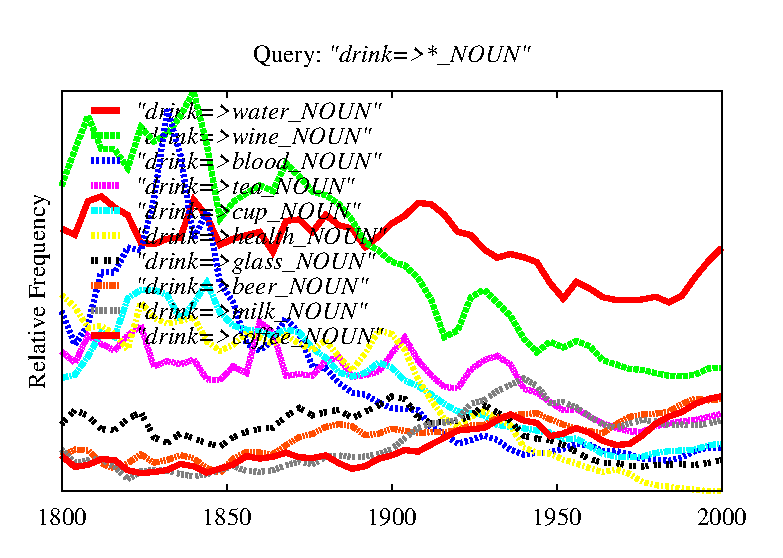
\includegraphics[width=.48\textwidth]{graphs/drink}
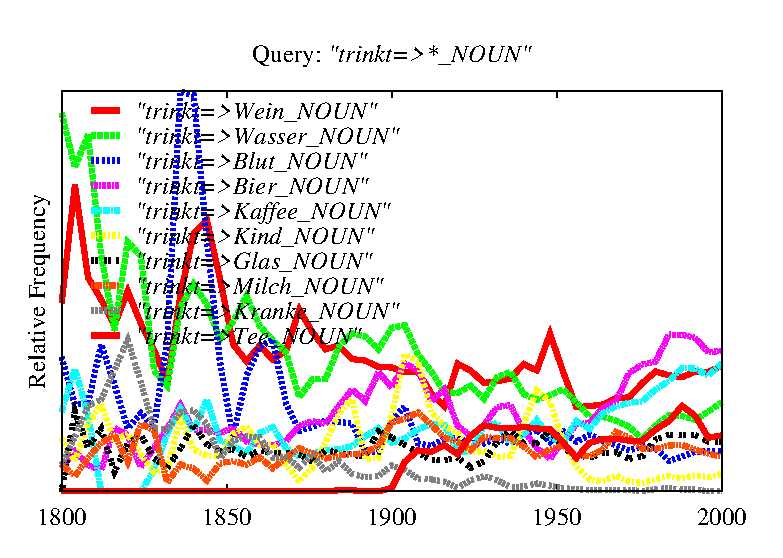
\includegraphics[width=.48\textwidth]{graphs/drink_GER}
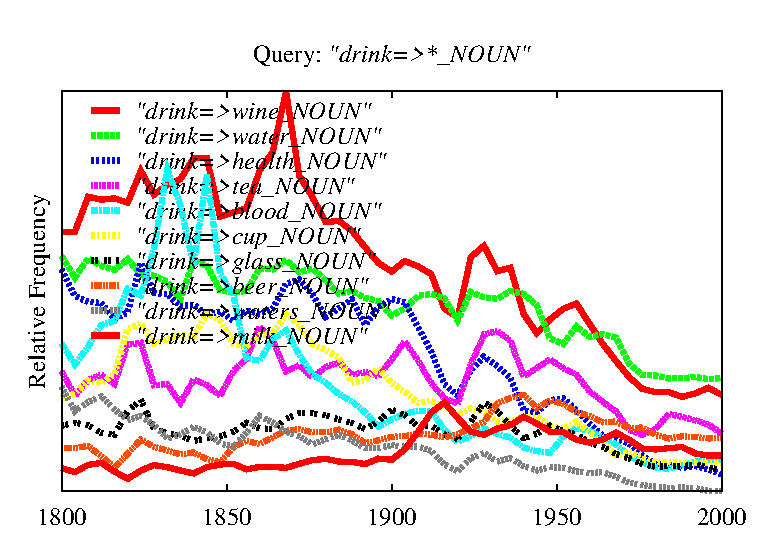
\includegraphics[width=.48\textwidth]{graphs/drink_UK}
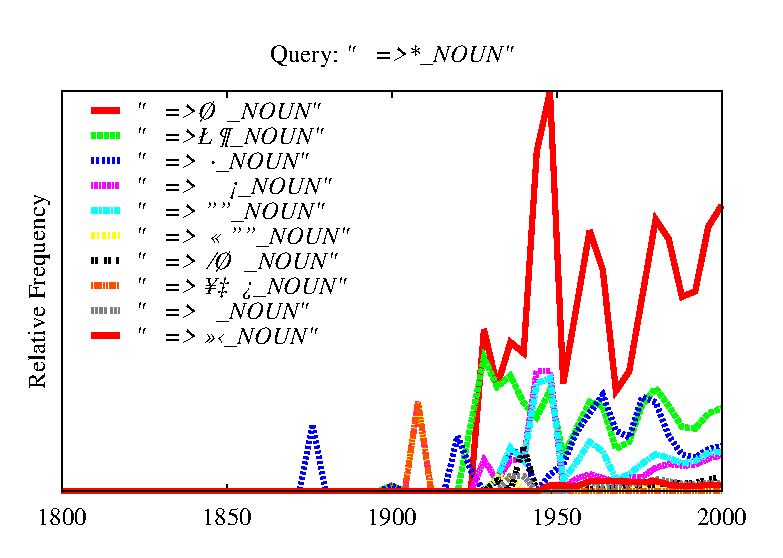
\includegraphics[width=.48\textwidth]{graphs/drink_CHI}
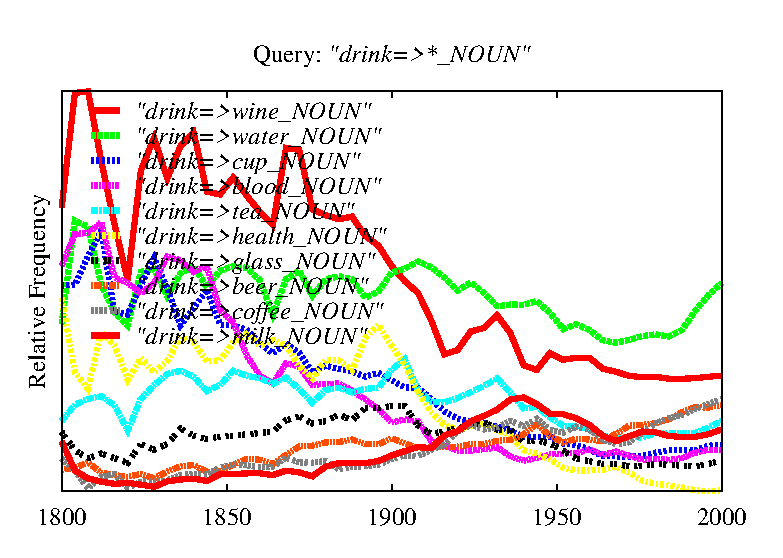
\includegraphics[width=.48\textwidth]{graphs/drink_USA}
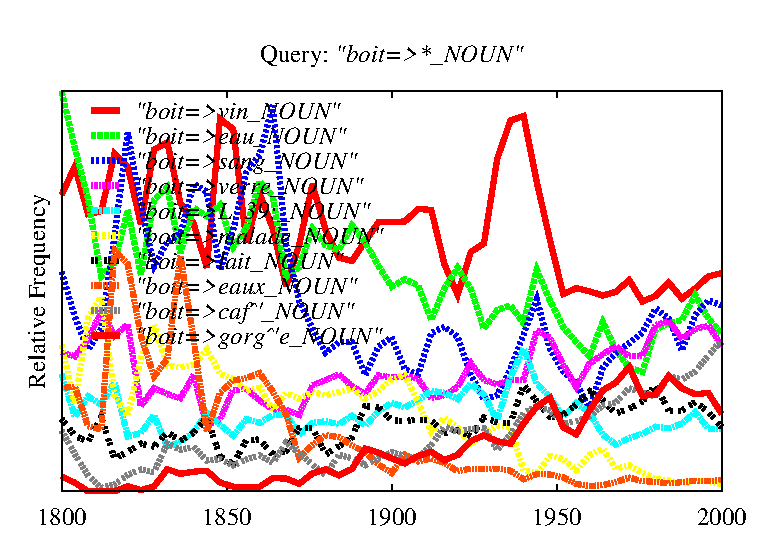
\includegraphics[width=.48\textwidth]{graphs/drink_FRE}
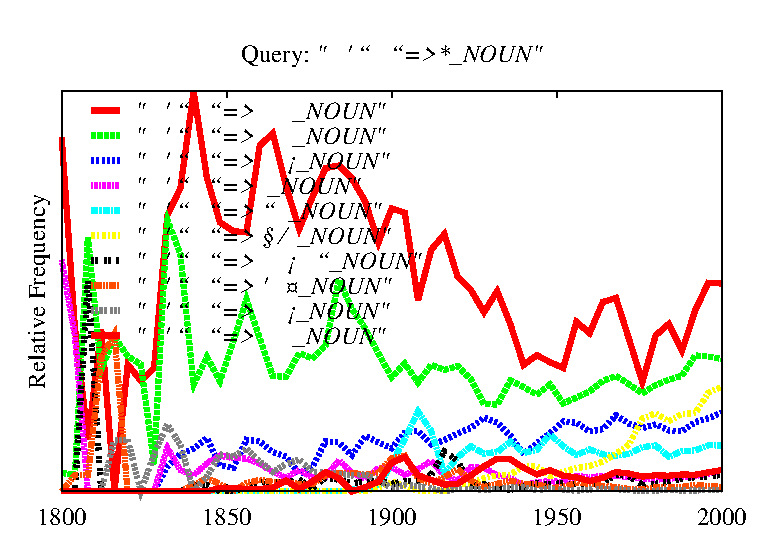
\includegraphics[width=.48\textwidth]{graphs/drink_HEB}
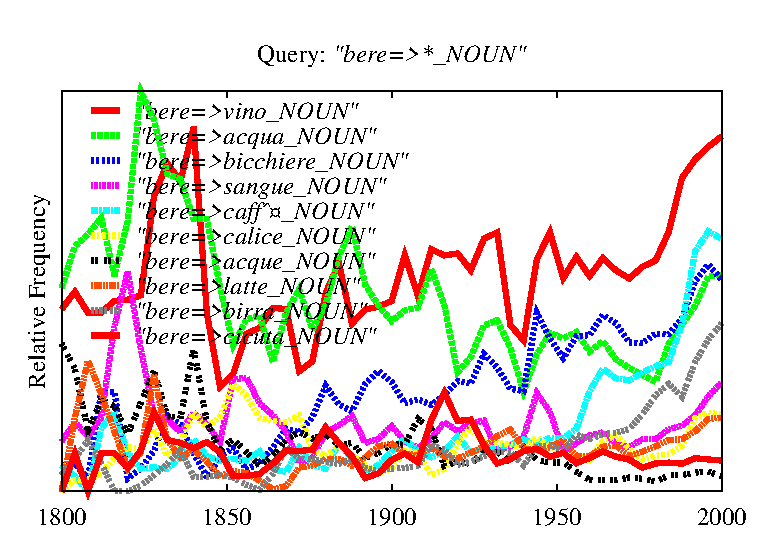
\includegraphics[width=.48\textwidth]{graphs/drink_ITA}
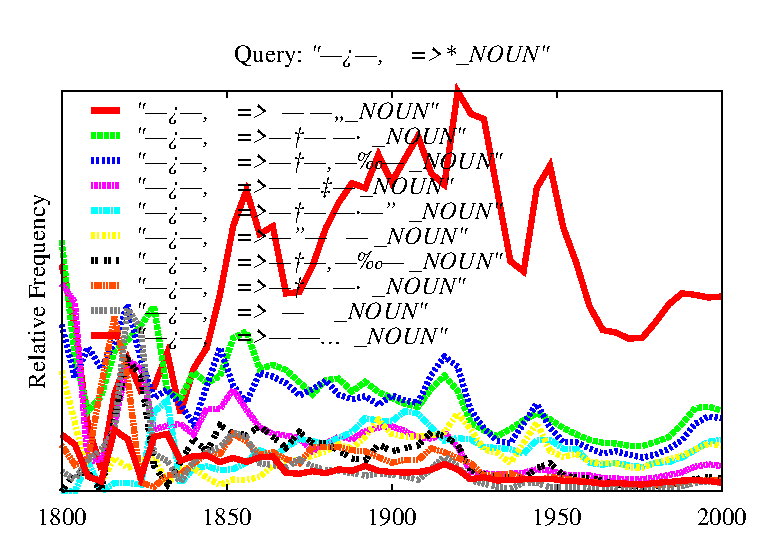
\includegraphics[width=.48\textwidth]{graphs/drink_RUS}
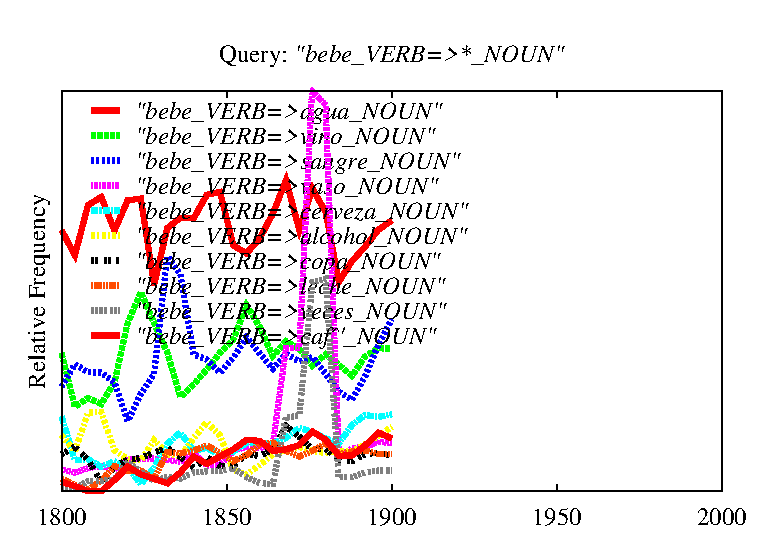
\includegraphics[width=.48\textwidth]{graphs/drink_SPA}}


\end{document}
